\documentclass[12pt]{article}

\usepackage{sbc-template}
\usepackage{amsmath, amsfonts, amssymb}
\usepackage{cite}
\usepackage{listings}
\usepackage{xcolor}
\usepackage[ruled,vlined,linesnumbered,portuguese]{algorithm2e}
\usepackage{graphicx, url}
\usepackage{float}
\usepackage{verbatim}
\usepackage[brazil]{babel}
\usepackage[utf8]{inputenc}
\usepackage[T1]{fontenc}
\usepackage{placeins}
\usepackage{hyperref}

\renewcommand{\footnotesize}{\scriptsize}
\hyphenpenalty=750

\pagestyle{plain}
\sloppy

% Configuração para listings
\lstset{
  basicstyle=\footnotesize\ttfamily,
  keywordstyle=\color{blue},
  stringstyle=\color{red},
  commentstyle=\color{green!60!black},
  frame=lines,
  numbers=left,
  numberstyle=\tiny\color{gray},
  breaklines=true,
  showstringspaces=false
}

\title{FLASC: Aprendizado Federado com Agrupamento Suave Adaptativo para Minimização do Impacto da Heterogeneidade de Dados}

\author{
  Pedro Gabriel do Valle Nogueira\inst{1}
}

\address{
  Programa de Pós-Graduação em Engenharia Eletrônica\\
  Universidade do Estado do Rio de Janeiro (UERJ) -- Rio de Janeiro, RJ -- Brasil
}

\begin{document}

\maketitle

\begin{resumo}
  O Aprendizado Federado (FL) enfrenta desafios devido à heterogeneidade estatística dos dados distribuídos.
  O método FLSC minimiza esse impacto ao permitir que clientes participem de múltiplos clusters simultaneamente,
  entretanto, utiliza parâmetros fixos e pesos uniformes.
  Este trabalho propõe o FLASC (\textit{Federated Learning with Adaptive Soft Clustering}),
  uma abordagem que introduz a seleção adaptativa de modelos baseada em um limiar de tolerância e a fusão ponderada pela perda local.
  Essa estratégia permite que o nível de participação e a influência de cada modelo se ajustem dinamicamente à distribuição de dados de cada cliente.
  Testes com o conjunto CIFAR-10 mostram que o FLASC atinge resultados similares ao estado da arte.
\end{resumo}

\begin{abstract}
  Federated Learning (FL) faces challenges due to statistical heterogeneity of distributed data.
  The FLSC method minimizes this impact by allowing clients to participate in multiple clusters simultaneously;
  however, it relies on fixed parameters and uniform weights.
  This work proposes FLASC (Federated Learning with Adaptive Soft Clustering),
  an approach that introduces adaptive model selection based on a tolerance threshold and weighted fusion through local loss.
  This strategy allows the participation level and the influence of each model to dynamically adjust to each client's data distribution.
  Tests with the CIFAR-10 dataset show that FLASC achieves results similar to the state-of-the-art.
\end{abstract}

\section{Introdução}

A crescente digitalização de serviços e a onipresença de dispositivos computacionais pessoais gera um volume de dados distribuídos sem precedentes,
o que impulsiona o desenvolvimento de soluções baseadas em aprendizado de máquina (ML) \cite{li2022federated, kim2023kfl}.
Em cenários convencionais, uma solução de ML exigiria a centralização dessas informações em um único servidor para o treinamento.
No entanto, a típica natureza sensível dos dados distribuídos, como é o caso na área da saúde,
impõe restrições de privacidade que impedem essa abordagem centralizada \cite{mcmahan2017communication, zhang2025lcfed}.

Para superar esse obstáculo, o Aprendizado Federado (do inglês, \textit{Federated Learning} -- FL)
surgiu como um paradigma onde cada cliente recebe uma cópia de um modelo global inicial,
realiza o treinamento com seus próprios dados e transmite apenas as atualizações do modelo \cite{mcmahan2017communication}.
O servidor, por sua vez, agrega essas atualizações com uma média ponderada (FedAvg) para criar uma nova versão do modelo global.
Esse processo se repete iterativamente por um determinado número de vezes até a convergência do modelo global \cite{mcmahan2017communication, li2022federated}.

Apesar dos avanços proporcionados pelo FL, sua eficácia é frequentemente desafiada pela heterogeneidade estatística dos dados nos clientes (dados não-IID).
Essa não uniformidade impacta negativamente a agregação,
tornando o modelo global subótimo para a maioria dos participantes \cite{ghosh2020efficient, briggs2020federated}.

Para mitigar esse impacto, uma linha de pesquisa proeminente foca no Aprendizado Federado Clusterizado
(do inglês, \textit{Clustered FederatedLearning} -- CFL).
A intuição por trás do CFL é agrupar clientes com distribuições de dados semelhantes
e treinar modelos especializados para cada grupo \cite{ghosh2020efficient, briggs2020federated, zhang2025lcfed}.
Essa abordagem tem demonstrado melhorar significativamente o desempenho em ambientes altamente heterogêneos \cite{li2022federated, kim2023kfl}.

Briggs et al. \cite{briggs2020federated} introduziram o FL+HC,
que aplica agrupamento hierárquico sobre a distância euclidiana dos pesos das atualizações.
A principal limitação dessa estratégia reside no fato de que,
uma vez que o modelo é cindido em clusters independentes,
a troca de conhecimento entre eles é permanentemente interrompida.
Essa segmentação estrita impede que clientes em clusters distintos,
mas com características latentes comuns,
continuem a se beneficiar de uma base de conhecimento compartilhada.

Buscando otimizar o momento da clusterização,
o método K-FL \cite{kim2023kfl} emprega um Filtro de Kalman para monitorar a tendência da acurácia e decidir o instante ideal para o agrupamento.
Apesar da inovação no uso de filtros estocásticos para lidar com o ruído das atualizações,
o K-FL ainda mantém a premissa de fronteiras rígidas (\textit{hard boundaries}),
onde um dispositivo é sumariamente excluído de um cluster caso sua performance divirja da média,
uma decisão que pode ser prematura em cenários de alta variância nos dados.

Para mitigar o \textit{overhead} de comunicação,
Zhang et al. \cite{zhang2025lcfed} propuseram o LCFed,
que utiliza a divisão do modelo (\textit{model splitting}) e aproximações de baixo posto (\textit{low-rank}) para calcular similaridades de forma eficiente.
No entanto, o LCFed ainda restringe a decisão final do cliente a um único submodelo,
limitando a expressividade da personalização em casos onde o perfil de dados do cliente transita entre diferentes distribuições.

No algoritmo IFCA, proposto por Ghosh et al. \cite{ghosh2020efficient},
o servidor mantém múltiplos modelos globais e os transmite aos clientes.
Cada participante avalia os modelos recebidos e seleciona aquele que minimiza sua perda empírica local para realizar o treinamento.
Essa abordagem exige que o cliente se vincule estritamente a um único modelo por rodada,
o que pode negligenciar conhecimento potencialmente útil dos modelos de outros clusters.

Finalmente, o Aprendizado Federado com Agrupamento Suave (FLSC),
apresentado por Li et al. \cite{li2022federated}, possibilitou que um cliente pertença a múltiplos clusters simultaneamente.
Graças a isso, o FLSC demonstrou capturar melhor a natureza dos dados reais~\cite{...}.
Contudo, o método obriga cada cliente a participar de exatamente $N$ clusters, sendo $N$ um hiperparâmetro.
Além disso, o FLSC não considera a possibilidade de que o peso de participação do cliente em cada um dos $N$ clusters possa ser diferente.

Para superar essas limitações, este trabalho propõe o FLASC (\textit{Federated Learning with Adaptive Soft Clustering}).
Diferente do FLSC, o FLASC permite que a quantidade de clusters integrados varie conforme a necessidade de cada cliente.
Além disso, ele propõe uma adaptação mais precisa e robusta à heterogeneidade dos dados ao
ponderar a contribuição de cada modelo de cluster proporcionalmente à sua afinidade com os dados locais.
O restante deste trabalho está organizado da seguinte forma:
a Seção \ref{sec:proposta} descreve detalhadamente o funcionamento do algoritmo FLASC;
a Seção \ref{sec:metodologia} apresenta a metodologia de avaliação e o ambiente experimental;
a Seção \ref{sec:resultados} expõe e discute os resultados obtidos;
e, finalmente, a Seção \ref{sec:conclusao} traz as considerações finais e propostas de trabalhos futuros.

\section{FLASC} \label{sec:proposta}

O algoritmo FLASC (\textit{Federated Learning with Adaptive Soft Clustering}) é uma proposta de melhoria do FLSC \cite{li2022federated}
que introduz um mecanismo mais flexível de atribuição de identidade de cluster.
O funcionamento do FLASC pode ser decomposto em três fases principais: inicialização,
processamento adaptativo no cliente e agregação por cluster no servidor.

\subsection{Inicialização e Distribuição}

O servidor mantém um conjunto de $K$ modelos globais de cluster $\mathcal{W}_t = \{W_{1,t}, W_{2,t}, \dots, W_{K,t}\}$.
Em cada rodada de treinamento $t$, o servidor seleciona aleatoriamente uma fração de clientes participantes e transmite a eles todos os $K$ modelos.

\subsection{Seleção Adaptativa e Fusão no Cliente}

O cliente $c$ avalia a perda empírica de cada modelo utilizando seu conjunto de dados local $\mathcal{D}_c$.
A perda $L_{c,k}$ do $k$-ésimo modelo no cliente $c$ é obtida de acordo com a Equação \ref{eq:loss_eval}.
\begin{equation}
    L_{c,k} = \text{Loss}(W_{k,t}; \mathcal{D}_c) \label{eq:loss_eval}
\end{equation}

O processo de seleção depende da dispersão das perdas observadas.
Define-se $L_{min} = \min_k \{L_{c,k}\}$ e $L_{max} = \max_k \{L_{c,k}\}$. O algoritmo trata dois cenários fundamentais baseados na sensibilidade $\epsilon$:

\begin{enumerate}
    \item \textbf{Cenário de Indistinguibilidade ($L_{max} - L_{min} \leq \epsilon$):} Caso a diferença entre o melhor e o pior desempenho seja desprezível (ex: $\epsilon = 10^{-5}$), o cliente seleciona aleatoriamente um único modelo $k \in \{1, \dots, K\}$ para o treinamento local.

    \item \textbf{Cenário de Seleção Adaptativa ($L_{max} - L_{min} > \epsilon$):} As perdas são primeiramente normalizadas no intervalo $[0, 1]$ seguindo a Equação \ref{eq:normalization}:
    \begin{equation}
        \hat{L}_{c,k} = \frac{L_{c,k} - L_{min}}{L_{max} - L_{min}} \label{eq:normalization}
    \end{equation}

    O conjunto de índices $S_c$ dos modelos selecionados é determinado pelo critério de tolerância $\rho \in [0, 1]$, conforme definido na Equação \ref{eq:selection_set}:
    \begin{equation}
        S_c = \{k \in \{1, \dots, K\} \mid \hat{L}_{c,k} \leq \rho\} \label{eq:selection_set}
    \end{equation}
\end{enumerate}

Para a fusão local, o FLASC atribui pesos $\alpha_{c,k}$ que priorizam modelos com melhor ajuste. Define-se inicialmente o valor de suporte $v_{c,k} = 1 - \hat{L}_{c,k}$. O peso final de cada modelo selecionado é obtido pela Equação \ref{eq:fusion_weights}:
\begin{equation}
    \alpha_{c,k} = \frac{v_{c,k}}{\sum_{j \in S_c} v_{c,j}} \label{eq:fusion_weights}
\end{equation}

A Listagem \ref{code:flasc_select} apresenta a implementação em Python da lógica de seleção adaptativa, destacando a transição entre os modelos matemáticos e a execução prática no cliente.

\begin{lstlisting}[language=Python, caption={Lógica de seleção adaptativa no cliente FLASC.}, label={code:flasc_select}, frame=lines, numbers=left, basicstyle=\footnotesize\ttfamily, keywordstyle=\color{blue}]
def select_models(losses, rho, epsilon=1e-5):
    lmin, lmax = min(losses), max(losses)

    # Caso de indistinguibilidade
    if (lmax - lmin) <= epsilon:
        idx = np.random.choice(len(losses))
        return [idx], [1.0]

    # Selecao baseada em tolerancia (rho)
    selected, raw_weights = [], []
    for i, loss in enumerate(losses):
        norm_l = (loss - lmin) / (lmax - lmin)
        if norm_l <= rho:
            selected.append(i)
            # v = 1 - norm_l (melhor perda = maior peso)
            raw_weights.append(1.0 - norm_l)

    # Normalizacao dos pesos de fusao
    total = sum(raw_weights)
    weights = [w / total for w in raw_weights]
    return selected, weights
\end{lstlisting}

O modelo de partida para o treinamento local, $W_{c,t}^{start}$, é construído através da combinação convexa dos modelos selecionados, conforme a Equação \ref{eq:convex_comb}:
\begin{equation}
    W_{c,t}^{start} = \sum_{k \in S_c} \alpha_{c,k} W_{k,t} \label{eq:convex_comb}
\end{equation}
Após a inicialização por fusão, o cliente realiza o treinamento local por $E$ épocas, resultando em um modelo atualizado $W_{c,t}^{end}$. O cliente, então, reporta ao servidor o modelo $W_{c,t}^{end}$ e o conjunto de identificadores $S_c$.

\subsection{Agregação por Cluster}

No servidor, os modelos globais são atualizados de forma independente. Para cada cluster $k \in \{1, \dots, K\}$, a agregação considera apenas os clientes que selecionaram o modelo $k$ em seu processo de fusão ($k \in S_c$), seguindo a Equação \ref{eq:aggregation}:
\begin{equation}
    W_{k,t+1} = \frac{\sum_{c: k \in S_c} n_c W_{c,t}^{end}}{\sum_{c: k \in S_c} n_c} \label{eq:aggregation}
\end{equation}
onde $n_c$ representa o número de amostras locais do cliente $c$. Essa arquitetura permite que os clusters evoluam de forma a representar especializações distintas nos dados, enquanto a natureza \textit{soft} da seleção adaptativa garante que os clientes possam se beneficiar de múltiplos domínios de conhecimento simultaneamente.

Em suma, o hiperparâmetro $\rho$ atua como um regulador da generalização do modelo. Valores de $\rho$ próximos a 0 aproximam o FLASC de abordagens de \textit{hard clustering} como o IFCA \cite{ghosh2020efficient}, onde apenas o melhor modelo é aproveitado. Por outro lado, valores próximos a 1 aproximam o comportamento do FLSC \cite{li2022federated}, permitindo uma fusão mais inclusiva. A natureza adaptativa do FLASC reside em permitir que essa decisão não seja global, mas sim tomada localmente por cada cliente com base na qualidade relativa dos modelos disponíveis frente aos seus dados específicos.

Em resumo, o fluxo operacional completo do FLASC é detalhado no Algoritmo \ref{alg:flasc}.

\begin{algorithm}[H]
    \SetAlgoLined
    \KwIn{Parâmetros iniciais $w_0$, tolerância $\rho$, sensibilidade $\epsilon$}
    \KwData{Conjuntos de dados locais $\{\mathcal{D}_c\}$ nos clientes}
    \BlankLine
    \textbf{Servidor:} Inicializa $K$ modelos de cluster $\mathcal{W}_0 = \{W_{1,0}, \dots, W_{K,0}\}$ com $w_0$\;
    \For{cada rodada $t = 0, 1, \dots, T$}{
        Servidor seleciona aleatoriamente um subconjunto de clientes $P_t$\;
        Servidor transmite $\mathcal{W}_t$ para todos os clientes em $P_t$\;
        \BlankLine
        \textbf{Cada cliente $c \in P_t$ em paralelo:}\;
        Avalia perdas locais $L_{c,k} = \text{Loss}(W_{k,t}; \mathcal{D}_c)$ para $k \in \{1, \dots, K\}$\;
        $L_{min} \leftarrow \min_k \{L_{c,k}\}$, $L_{max} \leftarrow \max_k \{L_{c,k}\}$\;
        \If{$L_{max} - L_{min} \leq \epsilon$}{
            $S_c \leftarrow \{ \text{índice aleatório de } \{1, \dots, K\} \}$\;
            $\alpha_{c,k} \leftarrow 1.0$ para $k \in S_c$\;
        }
        \Else{
            $\hat{L}_{c,k} \leftarrow \frac{L_{c,k} - L_{min}}{L_{max} - L_{min}}$ para cada $k$\;
            $S_c \leftarrow \{k \mid \hat{L}_{c,k} \leq \rho\}$\;
            $v_{c,k} \leftarrow 1 - \hat{L}_{c,k}$ para $k \in S_c$\;
            $\alpha_{c,k} \leftarrow v_{c,k} / \sum_{j \in S_c} v_{c,j}$ para $k \in S_c$\;
        }
        $W_{c,t}^{start} \leftarrow \sum_{k \in S_c} \alpha_{c,k} W_{k,t}$\;
        $W_{c,t}^{end} \leftarrow \text{TreinamentoLocal}(W_{c,t}^{start}, \mathcal{D}_c)$\;
        Envia $\{W_{c,t}^{end}, S_c\}$ para o servidor\;
        \BlankLine
        \textbf{Servidor:}\;
        \For{cada cluster $k \in \{1, \dots, K\}$}{
            $W_{k,t+1} \leftarrow \frac{\sum_{c: k \in S_c} n_c W_{c,t}^{end}}{\sum_{c: k \in S_c} n_c}$\;
        }
    }
    \caption{Algoritmo FLASC}
    \label{alg:flasc}
\end{algorithm}

\section{Configuração Experimental} \label{sec:experimentos}

Para avaliar o desempenho do FLASC, foram conduzidos experimentos utilizando o FLSC \cite{li2022federated} como linha de base.
O objetivo central da avaliação é qualificar o impacto de substituir o hiperparâmetro $N$ por $\rho$ (Veja a sessão ...).
Para garantir uma comparação equivalente entre os dois algoritmos,
variamos os hiperparâmetros $\rho$ e $N$ de forma correlacionada, conforme detalhado na Tabela \ref{tab:configs}.
Note que $N = 2$ significa que metade dos modelos serão selecionados.
Para reproduzir o equivalente com $\rho$,

\begin{table}[H]
\centering
\caption{Configuração dos hiperparâmetros de seleção para comparação.}
\label{tab:configs}
\begin{tabular}{lcc}
\hline
\textbf{Cenário} & \textbf{FLSC ($N$)} & \textbf{FLASC ($\rho$)} \\ \hline
Seleção Mínima   & 1                   & 0                       \\
Seleção Intermediária & 2                   & 0,5                     \\
Seleção Máxima (Inclusiva)   & 4                   & 1,0                     \\ \hline
\end{tabular}
\end{table}

Para os experimentos, utilizamos o conjunto de dados CIFAR-10,
que composto por 60.000 imagens coloridas de $32 \times 32$ pixels, distribuídas em 10 classes distintas.

A implementação do FLASC utiliza o framework Flower (\textit{v1.24.0}) \cite{beutel2020flower} com pytorch para orquestrar a simulação.
O código fonte completo, incluindo as estratégias de baseline e os scripts de reprodução,
está disponível publicamente em um repositório no GitHub\footnote{\url{https://github.com/nogueirapv/SimuAprendizadoFederado}}.

Quando ao particionamento dos dados, foi utilizado uma distribuição de Dirichlet com $\alpha = 0,5$
para refletir um cenário onde a distribuição de dados é desequilibrada.
Cada cliente divide sua partição local em 80\% para treinamento e 20\% para avaliação.

O modelo arquitetural adotado consiste em uma Rede Neural Convolucional (CNN) simples,
composta por duas camadas de convolução seguidas por camadas totalmente conectadas.
A primeira camada convolucional possui 6 filtros de tamanho $5 \times 5$,
enquanto a segunda possui 16 filtros de mesmo tamanho, ambas seguidas por operações de \textit{max-pooling} de $2 \times 2$.
As camadas densas subsequentes possuem 120, 84 e, finalmente, 10 neurônios na camada de saída, correspondendo às classes do CIFAR-10.
Foi utilizada a função de ativação ReLU em todas as camadas ocultas e o otimizador SGD com momento de $0,9$.
A função de perda adotada tanto para o treinamento local quanto para a avaliação de desempenho é a Entropia Cruzada (\textit{Cross-Entropy Loss}).

Configuramos o ambiente de simulação com 10 nós (clientes) participando de 10 rodadas de treinamento federado.
Em cada rodada, o servidor seleciona todos os clientes para o treinamento e metade deles para a etapa de avaliação.
Estabelecemos um conjunto de $K=4$ modelos globais para ambos os algoritmos.
Os parâmetros de treinamento local incluem 3 épocas, taxa de aprendizado de 0,001 e tamanho de lote de 32 amostras.

\subsection{Protocolo de Avaliação}

A avaliação ocorre ao final de cada rodada de treinamento.
Nesta etapa, o servidor transmite os $K$ modelos globais atualizados para os clientes selecionados.
Cada cliente avalia individualmente o desempenho de todos os $K$ modelos em seu conjunto de dados de teste local.
O cliente então identifica o modelo com o melhor desempenho (menor perda empírica) e reporta a acurácia e a perda deste modelo específico ao servidor.

O servidor agrega essas métricas calculando a média ponderada pelo número de amostras locais de cada cliente.
Este protocolo garante que a métrica final reflita a capacidade do sistema em oferecer, dentro do conjunto de clusters, pelo menos uma solução altamente especializada para cada distribuição de dados local encontrada na rede.
Dessa forma, avaliamos não apenas a convergência dos modelos, mas a eficácia da especialização promovida pelo agrupamento.

\section{Resultados} \label{sec:results}

Esta seção discute os resultados da avaliação de desempenho proposta na Seção~\ref{sec:experiment}.
Os gráficos mostram a média das cinco execuções independentes,
com as barras de erro indicando o desvio padrão.
A análise foca em como a substituição do parâmetro $N$ pelo parâmetro $\rho$ impacta as métricas de avaliação.

\subsection{Cenário de Seleção Mínima ($\rho=0$ e $N=1$)}

As Figuras~\ref{fig:acc_1} e \ref{fig:loss_1} ilustram a acurácia e a perda de avaliação para o cenário de seleção mínima.
Nesta configuração, o FLASC é restringido a selecionar apenas o modelo com a menor perda local ($\rho=0$),
replicando exatamente a lógica de seleção rígida do FLSC com $N=1$.
Os resultados apontam que, em um regime de seleção unitária,
o uso do $\rho$ mantém desempenho similar ao da linha de base conforme teorisado na Seção~\ref{sec:experiment}.

\begin{figure}[H]
    \centering
    \begin{minipage}{0.48\textwidth}
        \centering
        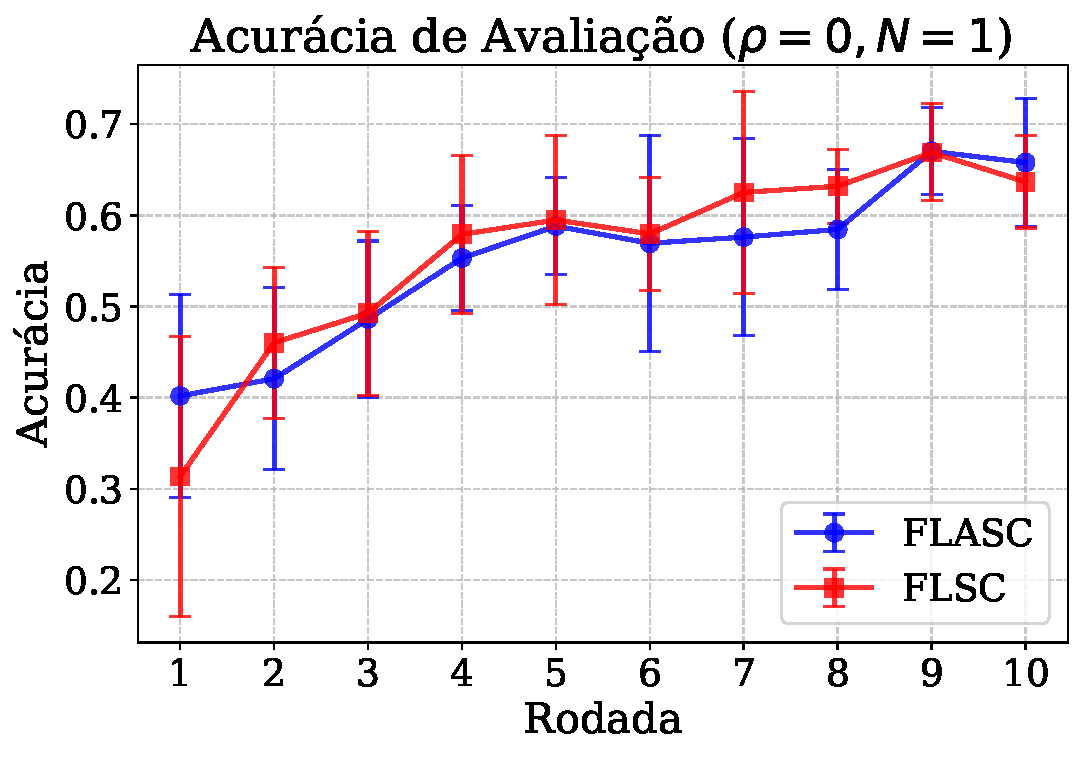
\includegraphics[width=\textwidth]{figs/eval_accuracy_1.pdf}
        \caption{Evolução da acurácia de avaliação no cenário de seleção mínima ($\rho=0, N=1$).}
        \label{fig:acc_1}
    \end{minipage}
    \hfill
    \begin{minipage}{0.48\textwidth}
        \centering
        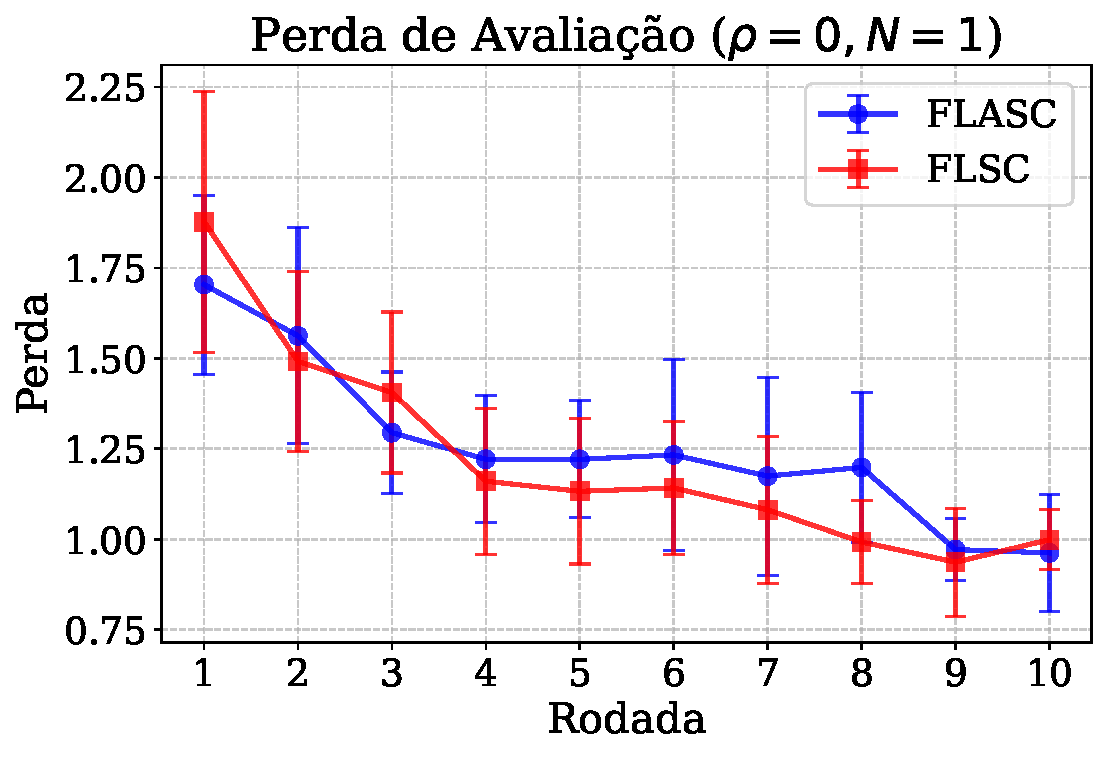
\includegraphics[width=\textwidth]{figs/eval_loss_1.pdf}
        \caption{Evolução da perda de avaliação no cenário de seleção mínima ($\rho=0, N=1$).}
        \label{fig:loss_1}
    \end{minipage}
\end{figure}

\subsection{Cenário de Seleção Intermediária ($\rho=0,5$ e $N=2$)}

No cenário intermediário, as Figuras~\ref{fig:acc_2} e \ref{fig:loss_2} mostram que o FLASC e o FLSC mantiveram comportamentos similares.
Havia a expectativa de que o limiar adaptativo $\rho$ permitisse um refinamento na seleção, 
filtrando modelos com desempenho marginal e favorecendo a estabilidade. 
Entretanto, a imposição de um número fixo de modelos ($N=2$) no FLSC não se mostrou prejudicial.

\begin{figure}[H]
    \centering
    \begin{minipage}{0.48\textwidth}
        \centering
        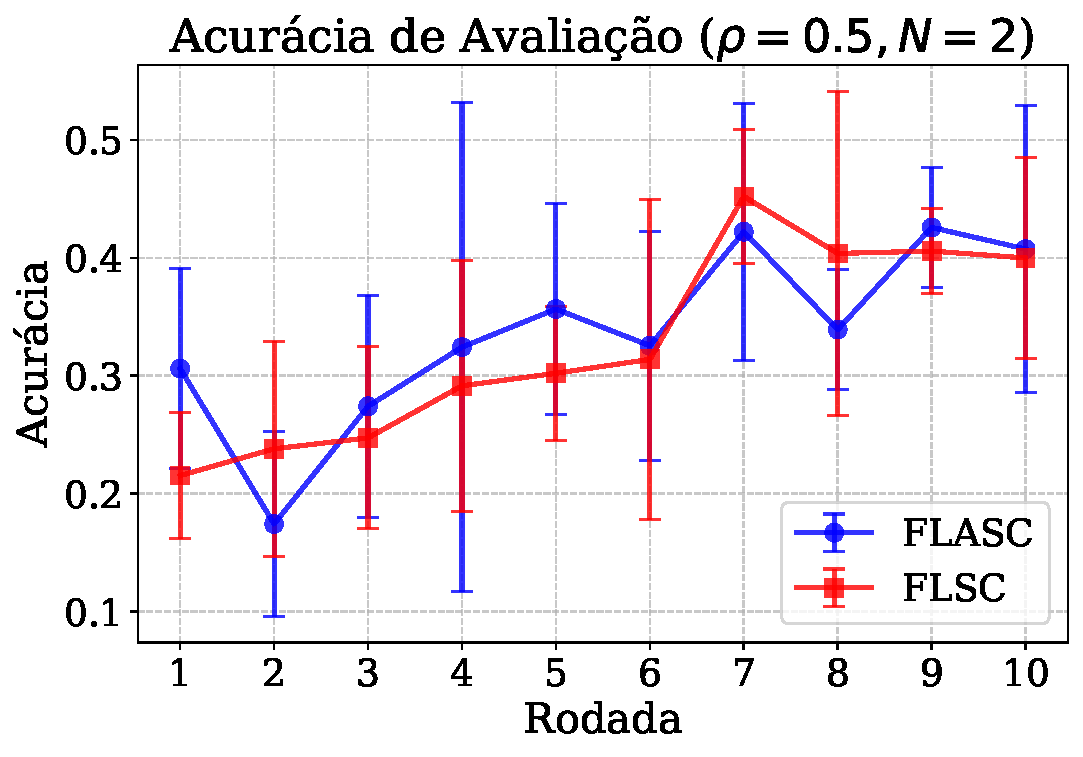
\includegraphics[width=\textwidth]{figs/eval_accuracy_2.pdf}
        \caption{Evolução da acurácia de avaliação no cenário intermediário ($\rho=0,5, N=2$).}
        \label{fig:acc_2}
    \end{minipage}
    \hfill
    \begin{minipage}{0.48\textwidth}
        \centering
        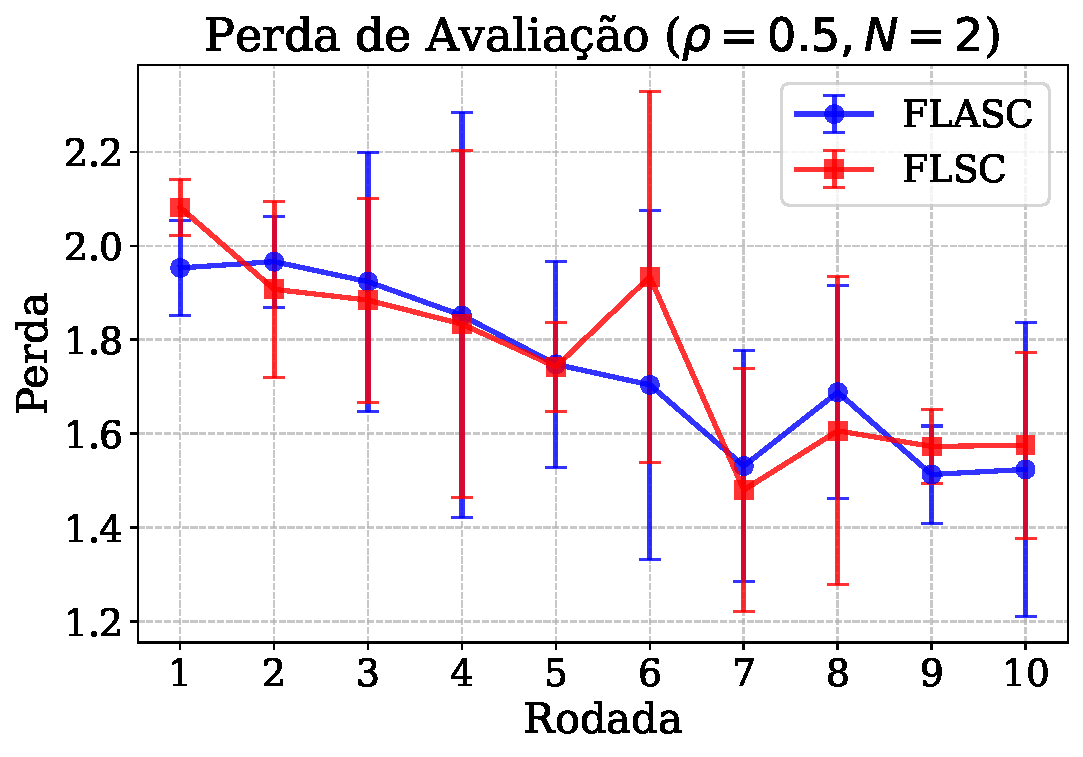
\includegraphics[width=\textwidth]{figs/eval_loss_2.pdf}
        \caption{Evolução da perda de avaliação no cenário intermediário ($\rho=0,5, N=2$).}
        \label{fig:loss_2}
    \end{minipage}
\end{figure}

\subsection{Cenário de Seleção Máxima ($\rho=1$ e $N=4$)}

Para o cenário de seleção máxima, as Figuras~\ref{fig:acc_3} e \ref{fig:loss_3}
revelam que a ponderação das perdas na fusão local não proporcionou ganhos significativos ao FLASC.
Embora a hipótese central fosse de que priorizar modelos com melhor adaptação local resultaria em uma convergência acelerada, 
os dados indicam que tanto a média ponderada quanto a média simples (FLSC) convergem para patamares de acurácia equivalentes.

\begin{figure}[H]
    \centering
    \begin{minipage}{0.48\textwidth}
        \centering
        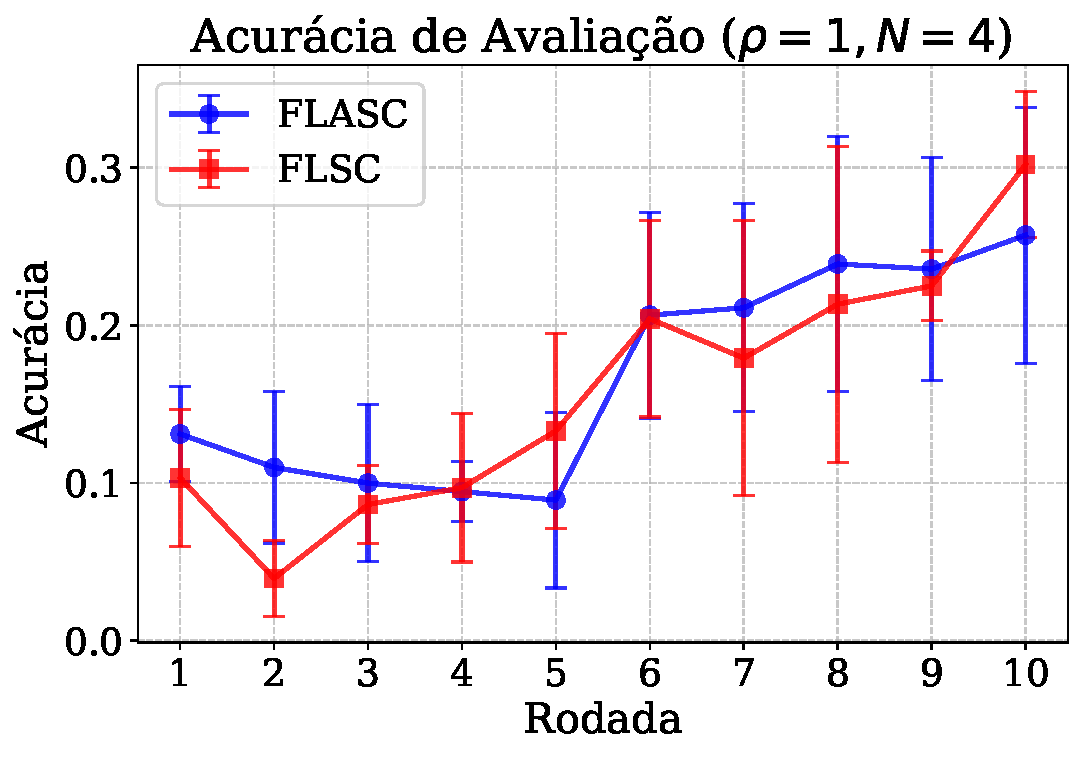
\includegraphics[width=\textwidth]{figs/eval_accuracy_3.pdf}
        \caption{Evolução da acurácia de avaliação no cenário de seleção máxima ($\rho=1, N=4$).}
        \label{fig:acc_3}
    \end{minipage}
    \hfill
    \begin{minipage}{0.48\textwidth}
        \centering
        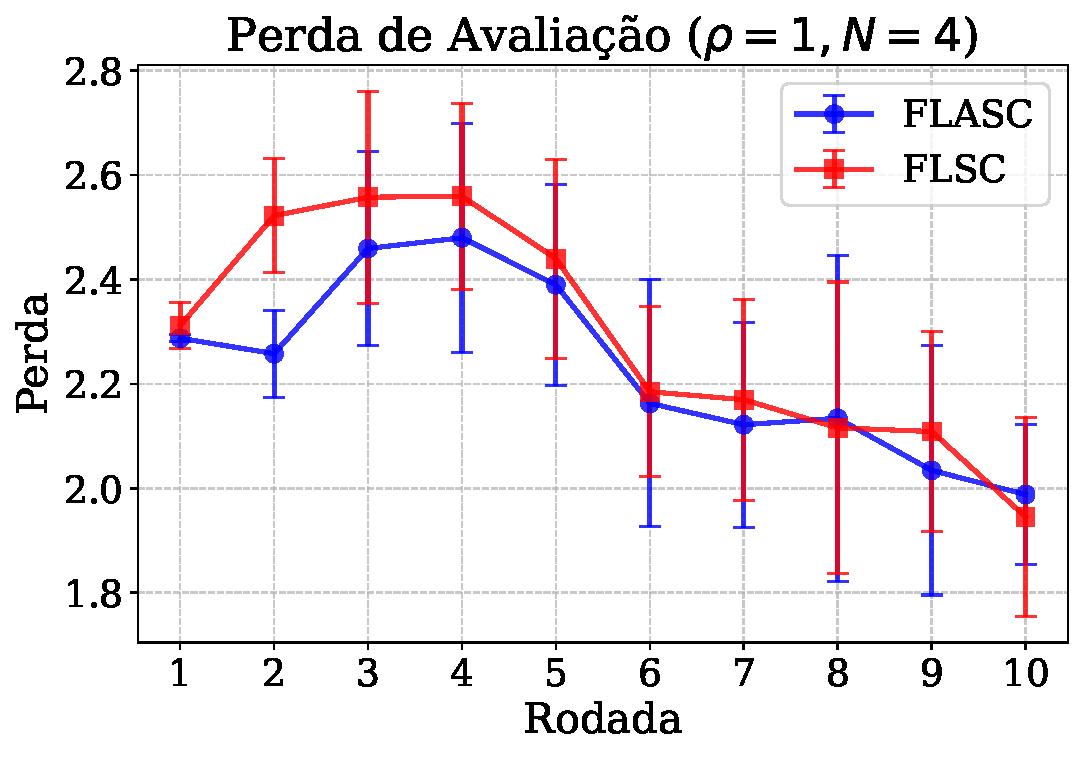
\includegraphics[width=\textwidth]{figs/eval_loss_3.pdf}
        \caption{Evolução da perda de avaliação no cenário de seleção máxima ($\rho=1, N=4$).}
        \label{fig:loss_3}
    \end{minipage}
\end{figure}

Em suma, os resultados mostram que a troca de parâmetros rígidos pelo 
mecanismo adaptativo proposto, embora ofereça maior flexibilidade teórica,
não resultou em diferença expressiva de desempenho no cenário experimental avaliado.

\section{Considerações Finais e Trabalhos Futuros} \label{sec:conclusion}

Neste trabalho, apresentamos o FLASC,
uma extensão do algoritmo FLSC que introduz um limiar adaptativo $\rho$ para a seleção de modelos e uma fusão local ponderada pela perda empírica.
A motivação central foi proporcionar maior flexibilidade de agrupamento
ao permitir que a quantidade e a influência de cada submodelo global fossem determinadas dinamicamente com base no desempenho local.

Os resultados experimentais conduzidos sobre o conjunto de dados CIFAR-10, em um cenário de heterogeneidade estatística,
revelaram que o FLASC mantém um desempenho equivalente ao FLSC.
Embora a hipótese inicial de que a seleção adaptativa e a ponderação de perdas se traduziria em ganhos significativos,
o FLASC demonstrou que a mudança de abordagem não foi inviável no cenário avaliado.

Como possibilidades para trabalhos futuros, propõem-se as seguintes frentes de investigação:

\begin{itemize}
    \item \textbf{Mais rodadas de treinamento:} Avaliar a convergência do FLASC em simulações de maior duração
    (ex: 20 a 50 rodadas) para verificar se vantagens da fusão adaptativa se revelam em treinamentos prolongados.
    \item \textbf{Exploração extensiva de hiperparâmetros:} Conduzir um estudo que explore mais o parâmetro $\rho$
    para avaliar melhor seu impacto no treinamento.
    \item \textbf{Diversificação do particionamento de dados:} Testar o algoritmo sob outras configurações de heterogeneidade.
\end{itemize}

\bibliographystyle{unsrt}
\bibliography{references}

\end{document}
